\documentclass[aspectratio=169,12pt,handout]{beamer}
\usepackage{pgfpages}
\pgfpagesuselayout{resize to}[letterpaper,landscape,border shrink=5mm]
\usetheme{Madrid}
\usecolortheme{default}
\usepackage{graphicx}
\usepackage{booktabs}
\usepackage{amsmath}

% Clean colors
\definecolor{binggreen}{RGB}{0,100,0}
\setbeamercolor{structure}{fg=binggreen}
\setbeamercolor{title}{fg=white,bg=binggreen}
\setbeamercolor{frametitle}{fg=white,bg=binggreen}

\setbeamertemplate{navigation symbols}{}
\setbeamertemplate{footline}{%
  \vspace*{4mm}\hfill\insertframenumber/\inserttotalframenumber\hspace{2mm}%
}

\hypersetup{pdfpagelayout=SinglePage}

\title{Shape vs.\ Magnitude}
\subtitle{Week of April 23}
\author{}
\institute{Binghamton University}
\date{April 2026}

\begin{document}

% ------------------------------------------------------------------
\begin{frame}
\titlepage
\end{frame}

% ------------------------------------------------------------------
\begin{frame}{Where We Left Off (April 16)}
\begin{columns}[T]
\begin{column}{0.55\textwidth}
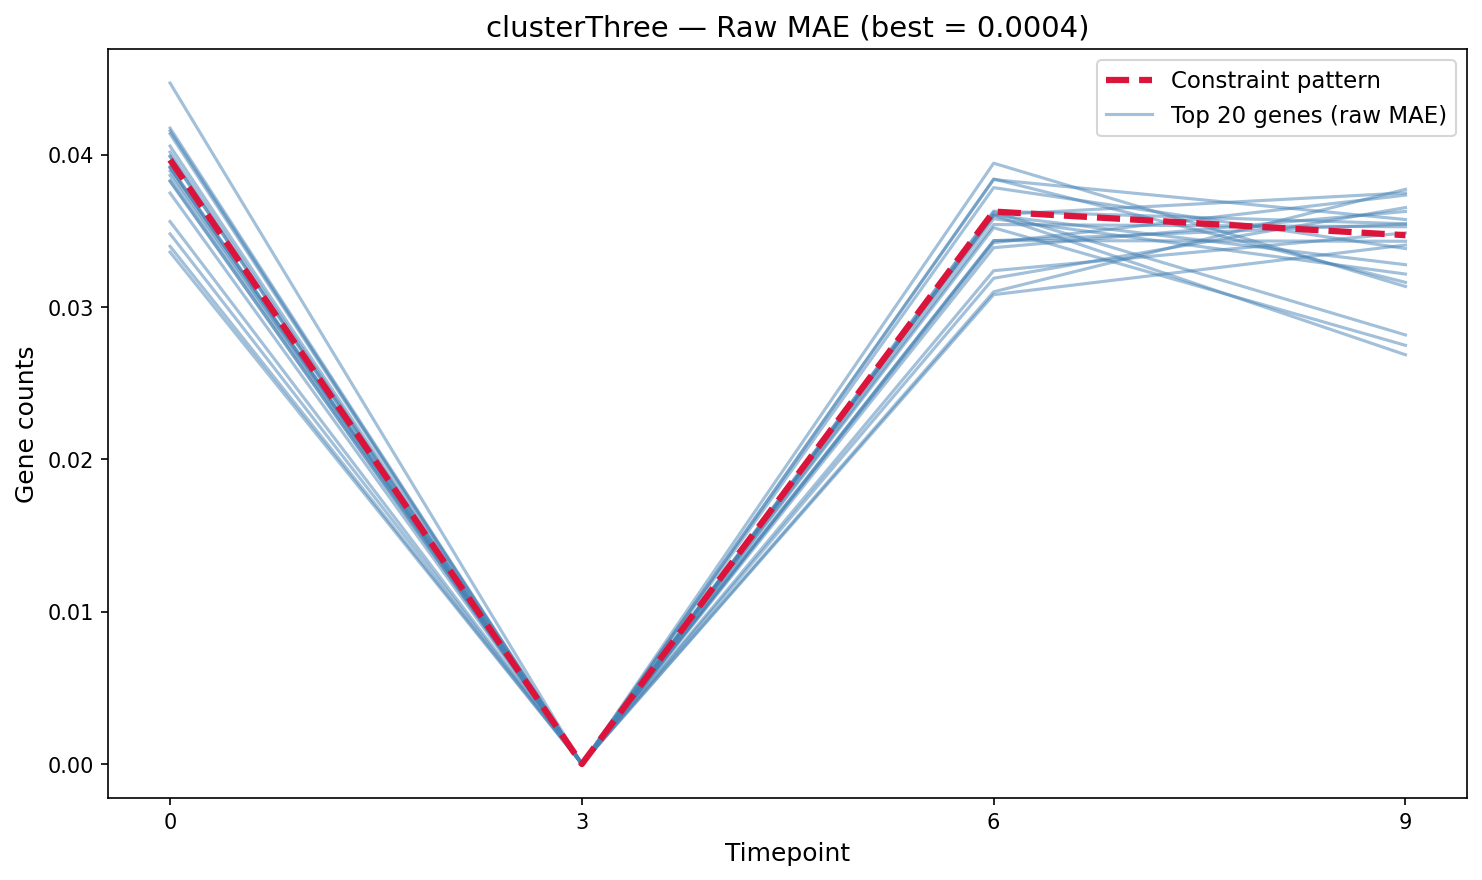
\includegraphics[width=\textwidth]{../Week of April 16th/plots/rawmae_clusterThree.png}
\end{column}
\begin{column}{0.42\textwidth}
\vspace{1em}
\textbf{Raw-space MAE} gave the best visual fit for clusters Two, Three, and Four.\\[0.5em]
The six prior methods all operate on \textit{normalized} data --- so they find genes with the right \textit{shape} at arbitrary expression levels.\\[0.5em]
\textbf{clusterOne} was the exception --- no genes at the pattern's magnitude also follow its spike shape.
\end{column}
\end{columns}
\end{frame}

% ------------------------------------------------------------------
\begin{frame}{All 4 Clusters --- Shape-Based vs.\ Magnitude-Based}
\begin{center}
\textbf{\textcolor{binggreen}{Shape-based gated ensemble}}\\[0.1em]
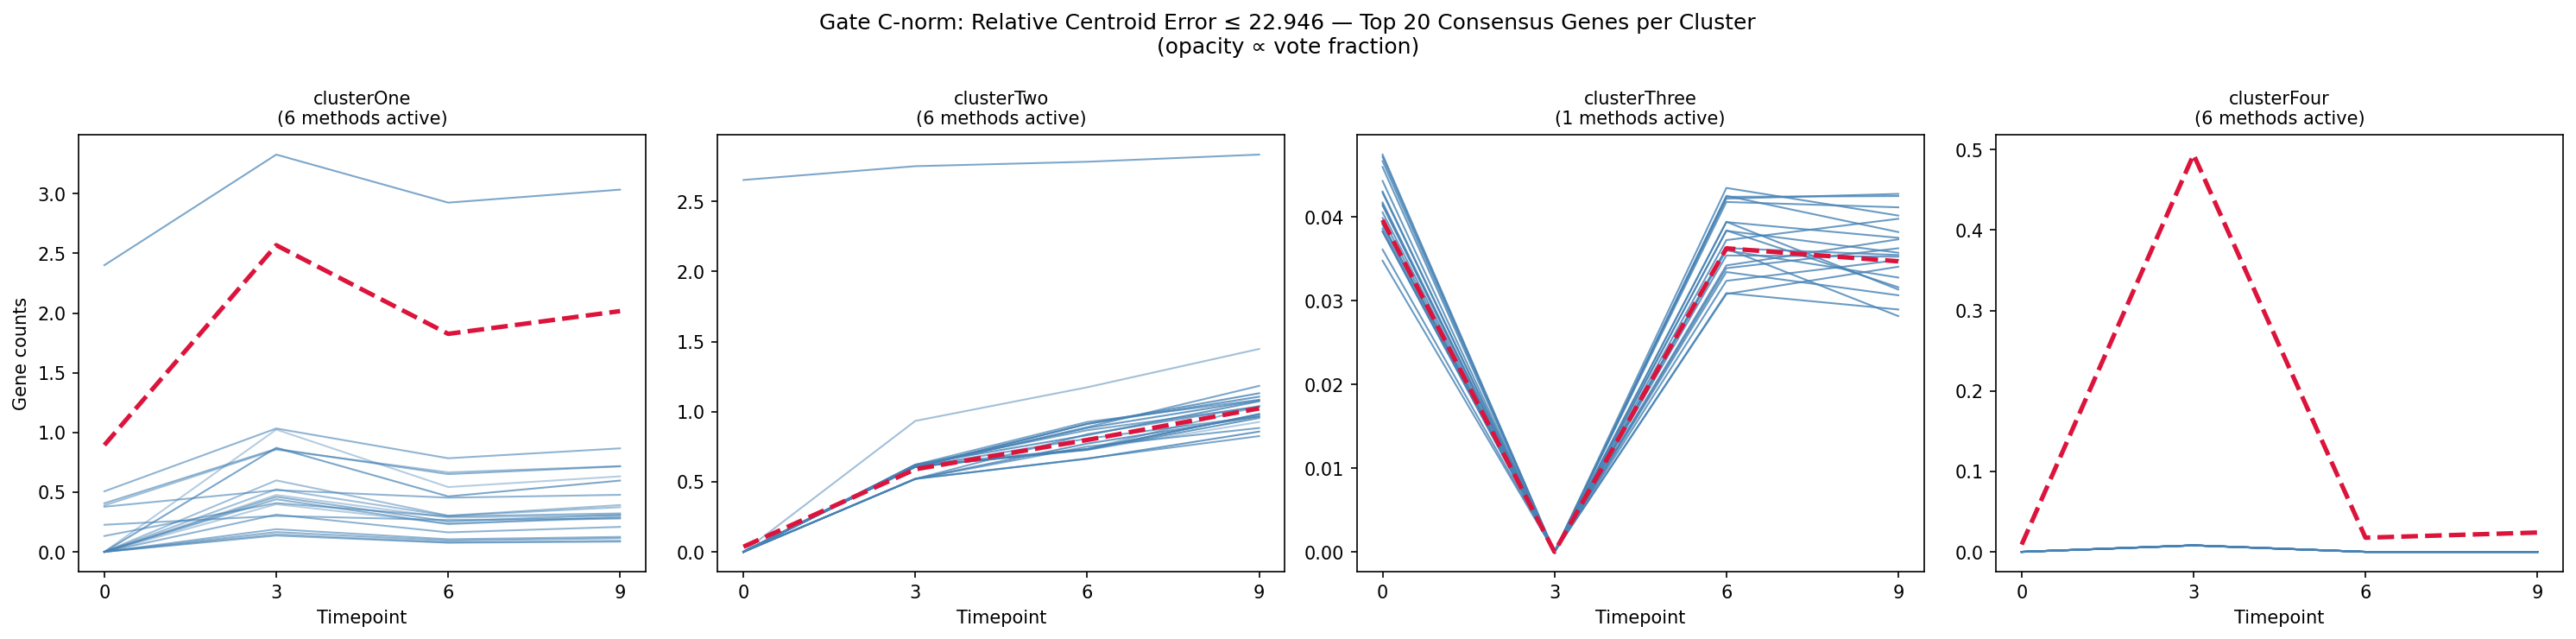
\includegraphics[width=\textwidth,height=0.36\textheight,keepaspectratio]{../Week of April 16th/plots/ensemble_gate_c_norm.png}\\[0.3em]
\textbf{\textcolor{binggreen}{Magnitude-based raw MAE}}\\[0.1em]
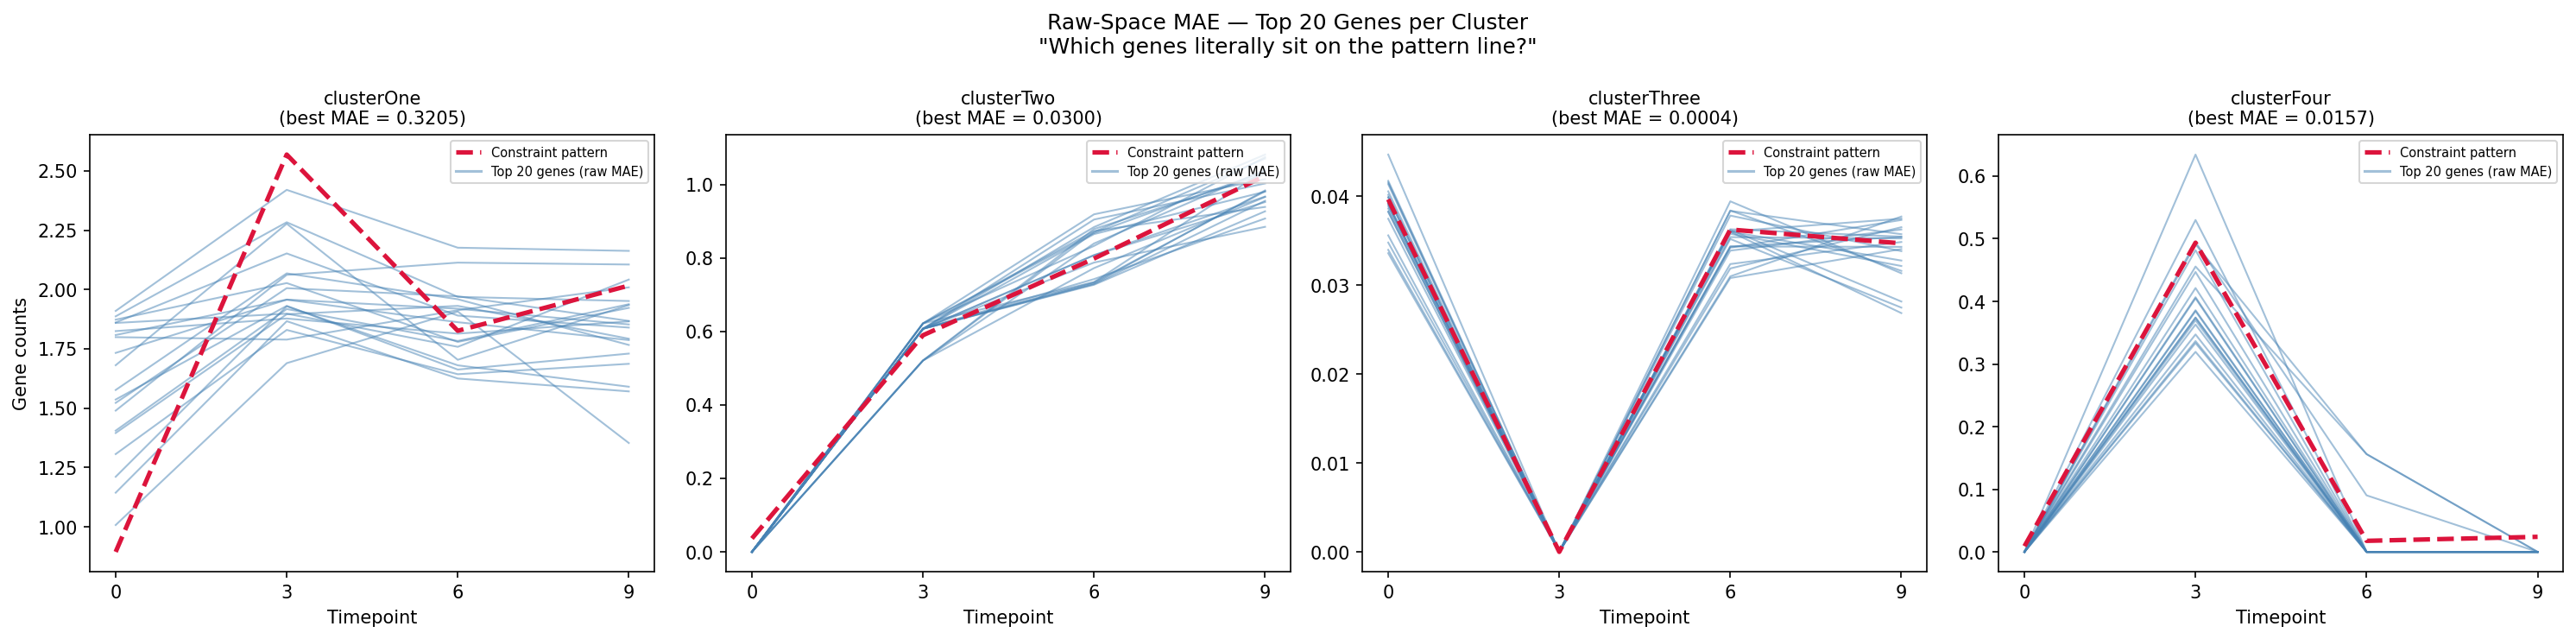
\includegraphics[width=\textwidth,height=0.36\textheight,keepaspectratio]{../Week of April 16th/plots/act3_raw_mae.png}
\end{center}
\end{frame}

% ------------------------------------------------------------------
\begin{frame}{Question}
\begin{center}
\Large
Is biological similarity a matter of\\[0.3em]
\textbf{\textcolor{binggreen}{direction of change}} (shape)\\[0.3em]
or \textbf{\textcolor{binggreen}{absolute expression level}} (magnitude)?
\end{center}
\end{frame}

% ------------------------------------------------------------------
\begin{frame}{The 4-Timepoint Problem}
\small
Each gene's trajectory has 3 transitions ($t_0 \to t_3$, $t_3 \to t_6$, $t_6 \to t_9$). Collapse each to its sign $\Rightarrow$ only $2^3 = 8$ possible ``shape classes.'' All 6 normalized-first methods also erase magnitude, so they're sorting $\sim\!17{,}856$ genes into 8 buckets on shape alone. Non-trivial fraction of genes share the constraint's sign class \textit{by accident}.
\normalsize
\begin{center}
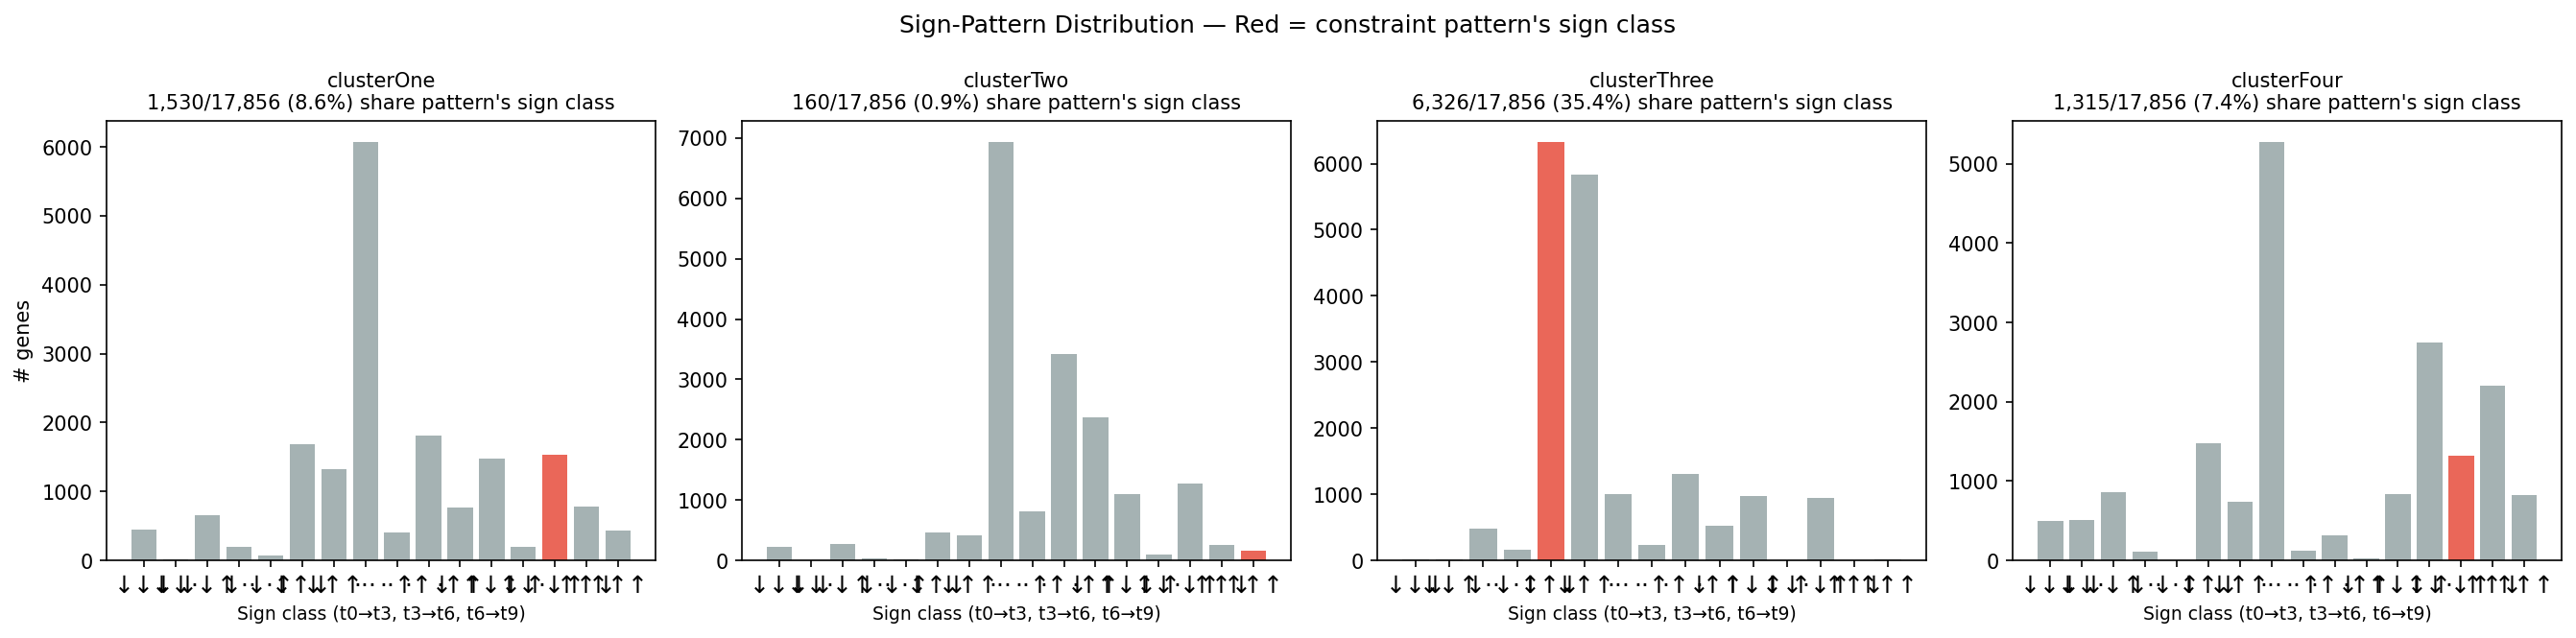
\includegraphics[width=0.98\textwidth]{plots/sign_pattern_distribution.png}
\end{center}
\end{frame}

% ------------------------------------------------------------------
\begin{frame}{clusterOne --- Spike Pattern, Moderate Magnitude}
\footnotesize
8.6\% of genes share the sign class \texttt{(+,-,+)}. The 6 normalized methods find spike-like genes mostly \textit{below} the pattern --- shape roughly right, magnitude off. Gated ensemble: 6/6 active (no method silenced). Raw MAE: genes sit at the right level but are flat. \textbf{\textcolor{binggreen}{Neither path is clean here.}}
\normalsize
\begin{center}
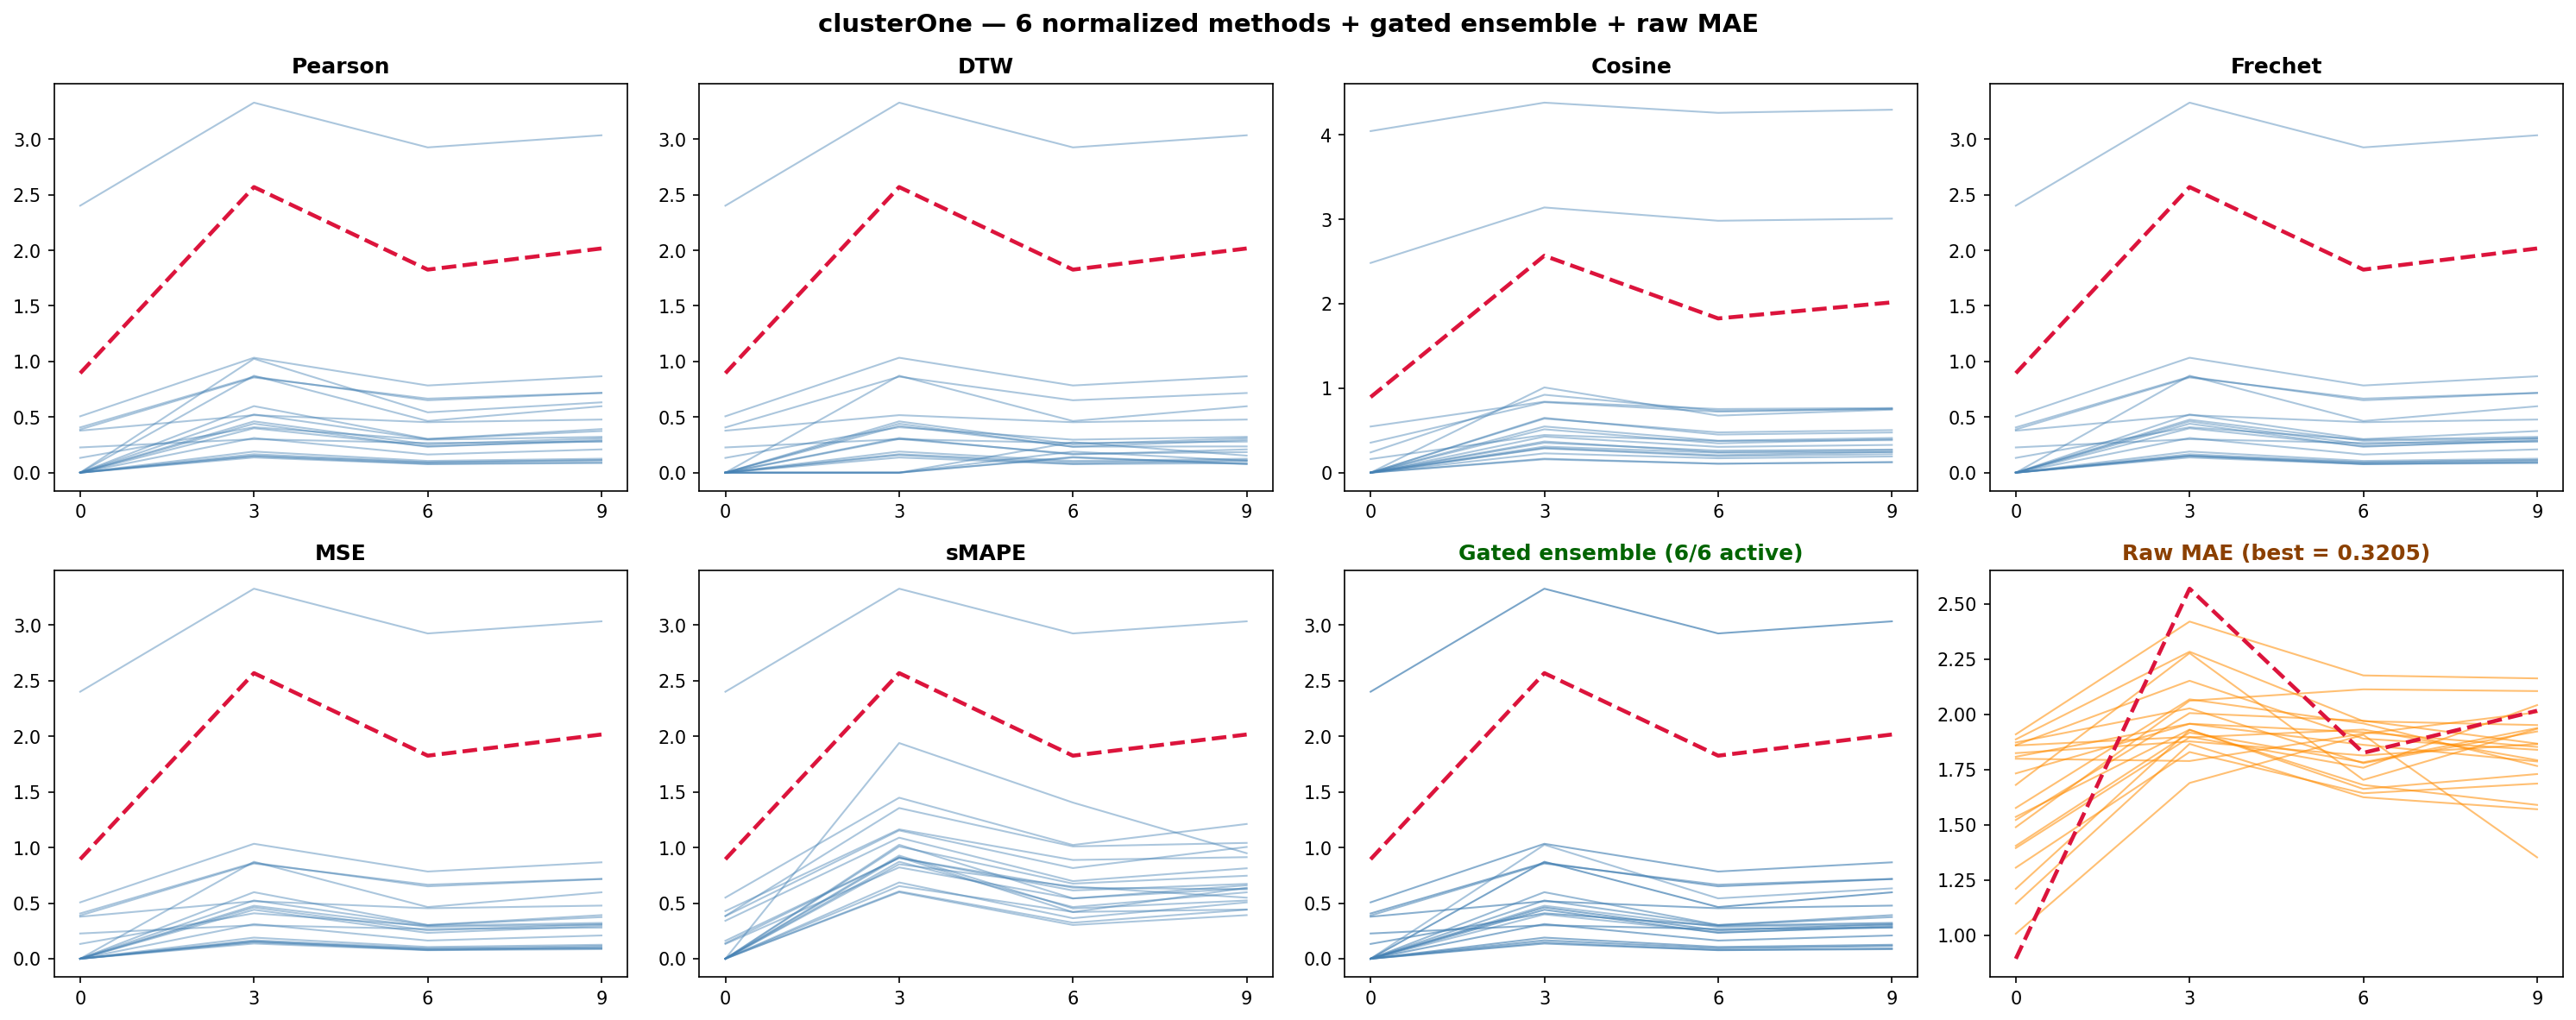
\includegraphics[width=\textwidth,height=0.78\textheight,keepaspectratio]{plots/eightways_clusterOne.png}
\end{center}
\end{frame}

% ------------------------------------------------------------------
\begin{frame}{clusterTwo --- Monotone Increase}
\footnotesize
Only 0.9\% of genes share \texttt{(+,+,+)} --- the rarest sign class, so shape is actually selective here. All 6 methods pick genes that hug both the shape and magnitude. Gated ensemble: 6/6 active, high consensus (RAB14, SYNGR1\ldots). Raw MAE: very tight fit (best $\approx 0.03$). \textbf{\textcolor{binggreen}{Both paths agree.}}
\normalsize
\begin{center}
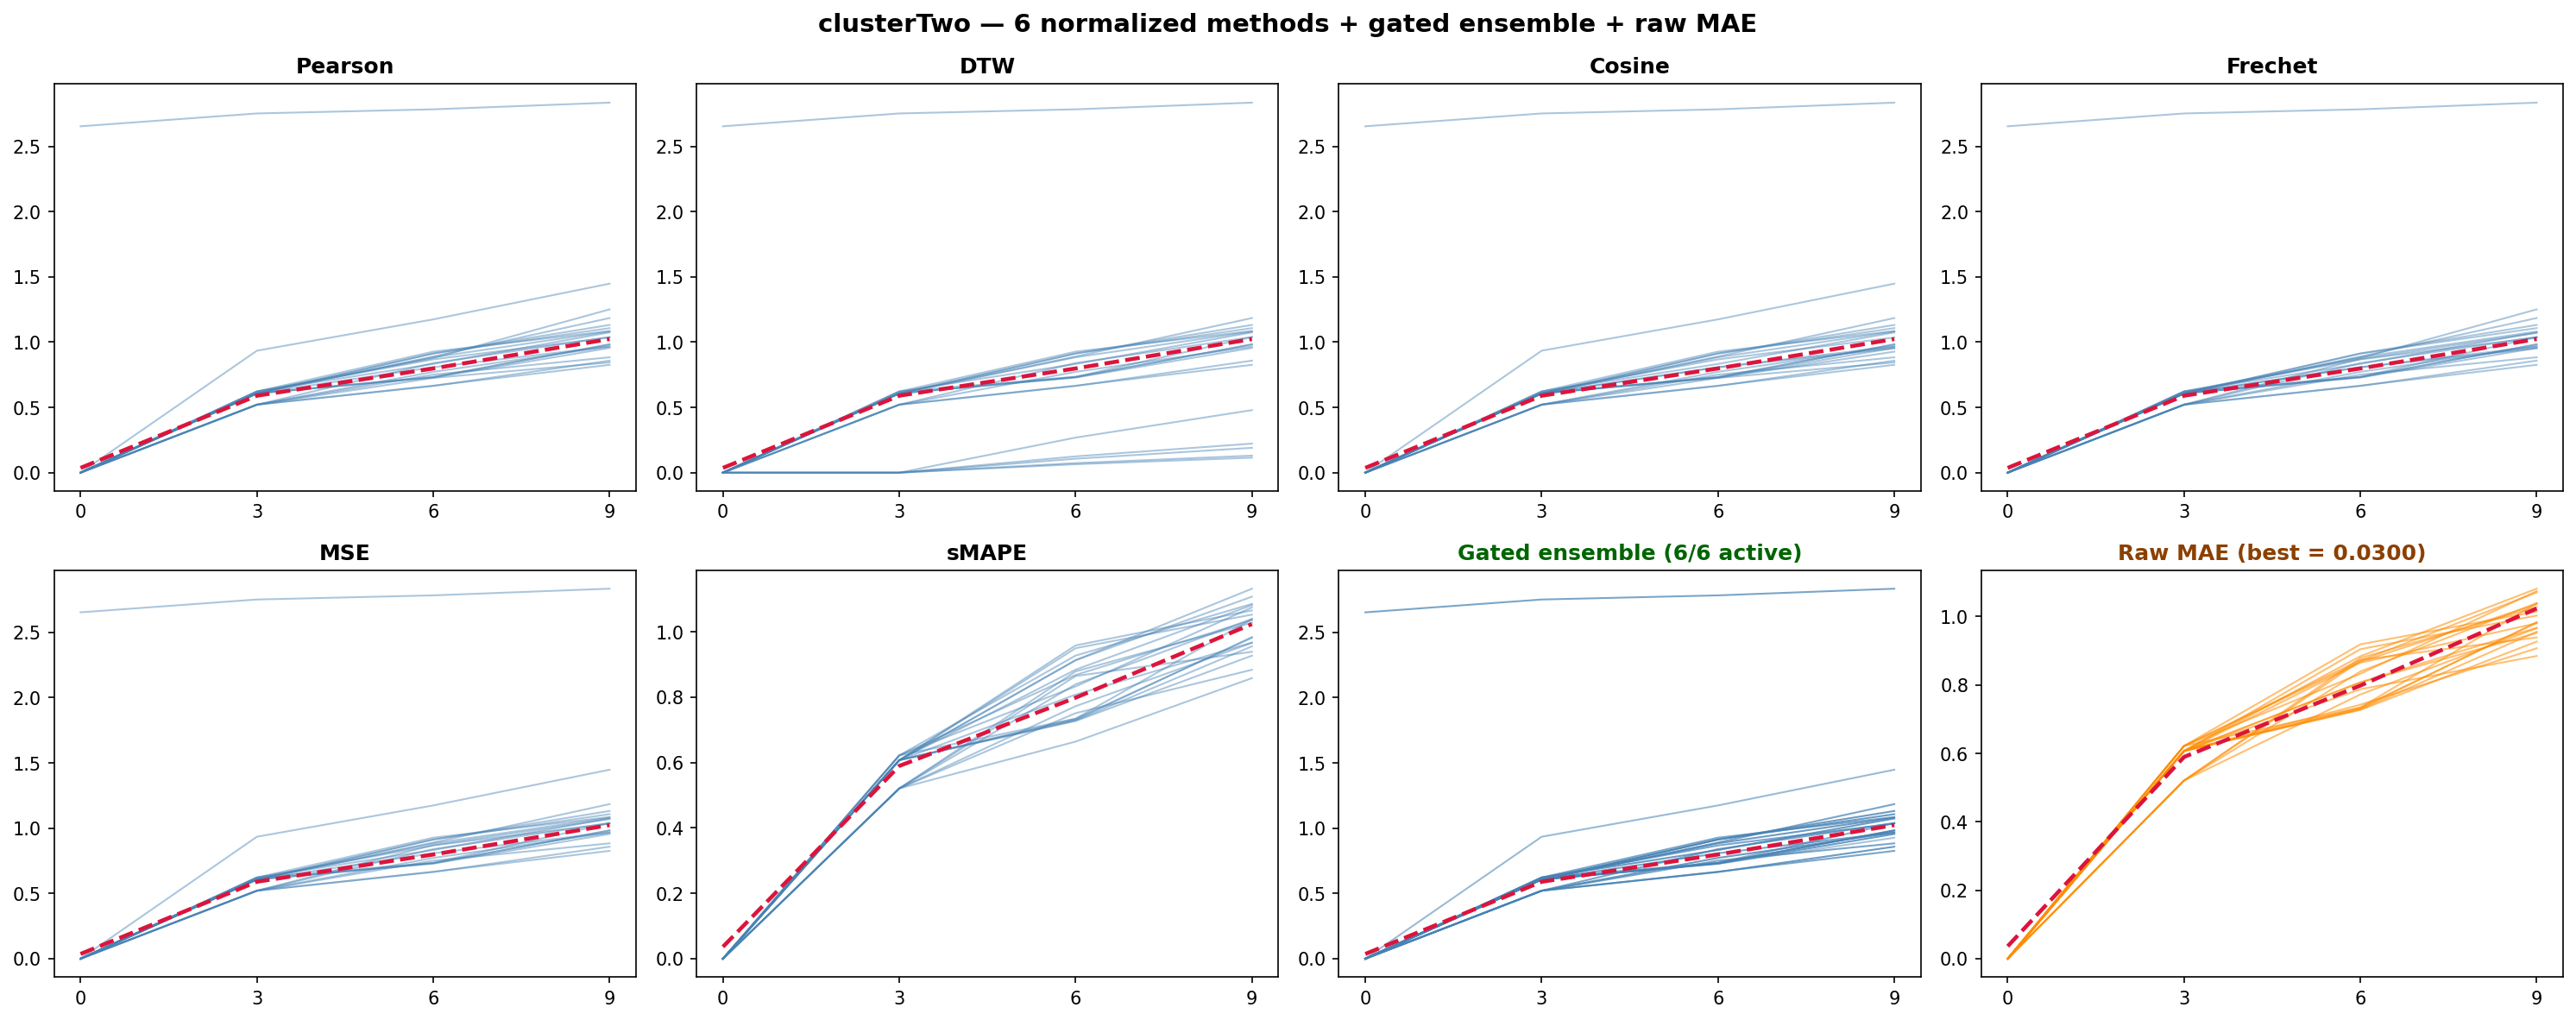
\includegraphics[width=\textwidth,height=0.78\textheight,keepaspectratio]{plots/eightways_clusterTwo.png}
\end{center}
\end{frame}

% ------------------------------------------------------------------
\begin{frame}{clusterThree --- Dip Pattern, Tiny Magnitude}
\footnotesize
35.4\% of genes share \texttt{(-,+,-)} --- the shape-based filter is weakest here. 5 of 6 normalized methods pick genes 10--40$\times$ \textit{above} the pattern (right shape, wrong level). Gated ensemble silences five --- only sMAPE survives (1/6 active). Raw MAE: genes sit directly on the pattern. \textbf{\textcolor{binggreen}{Magnitude looks closer.}}
\normalsize
\begin{center}
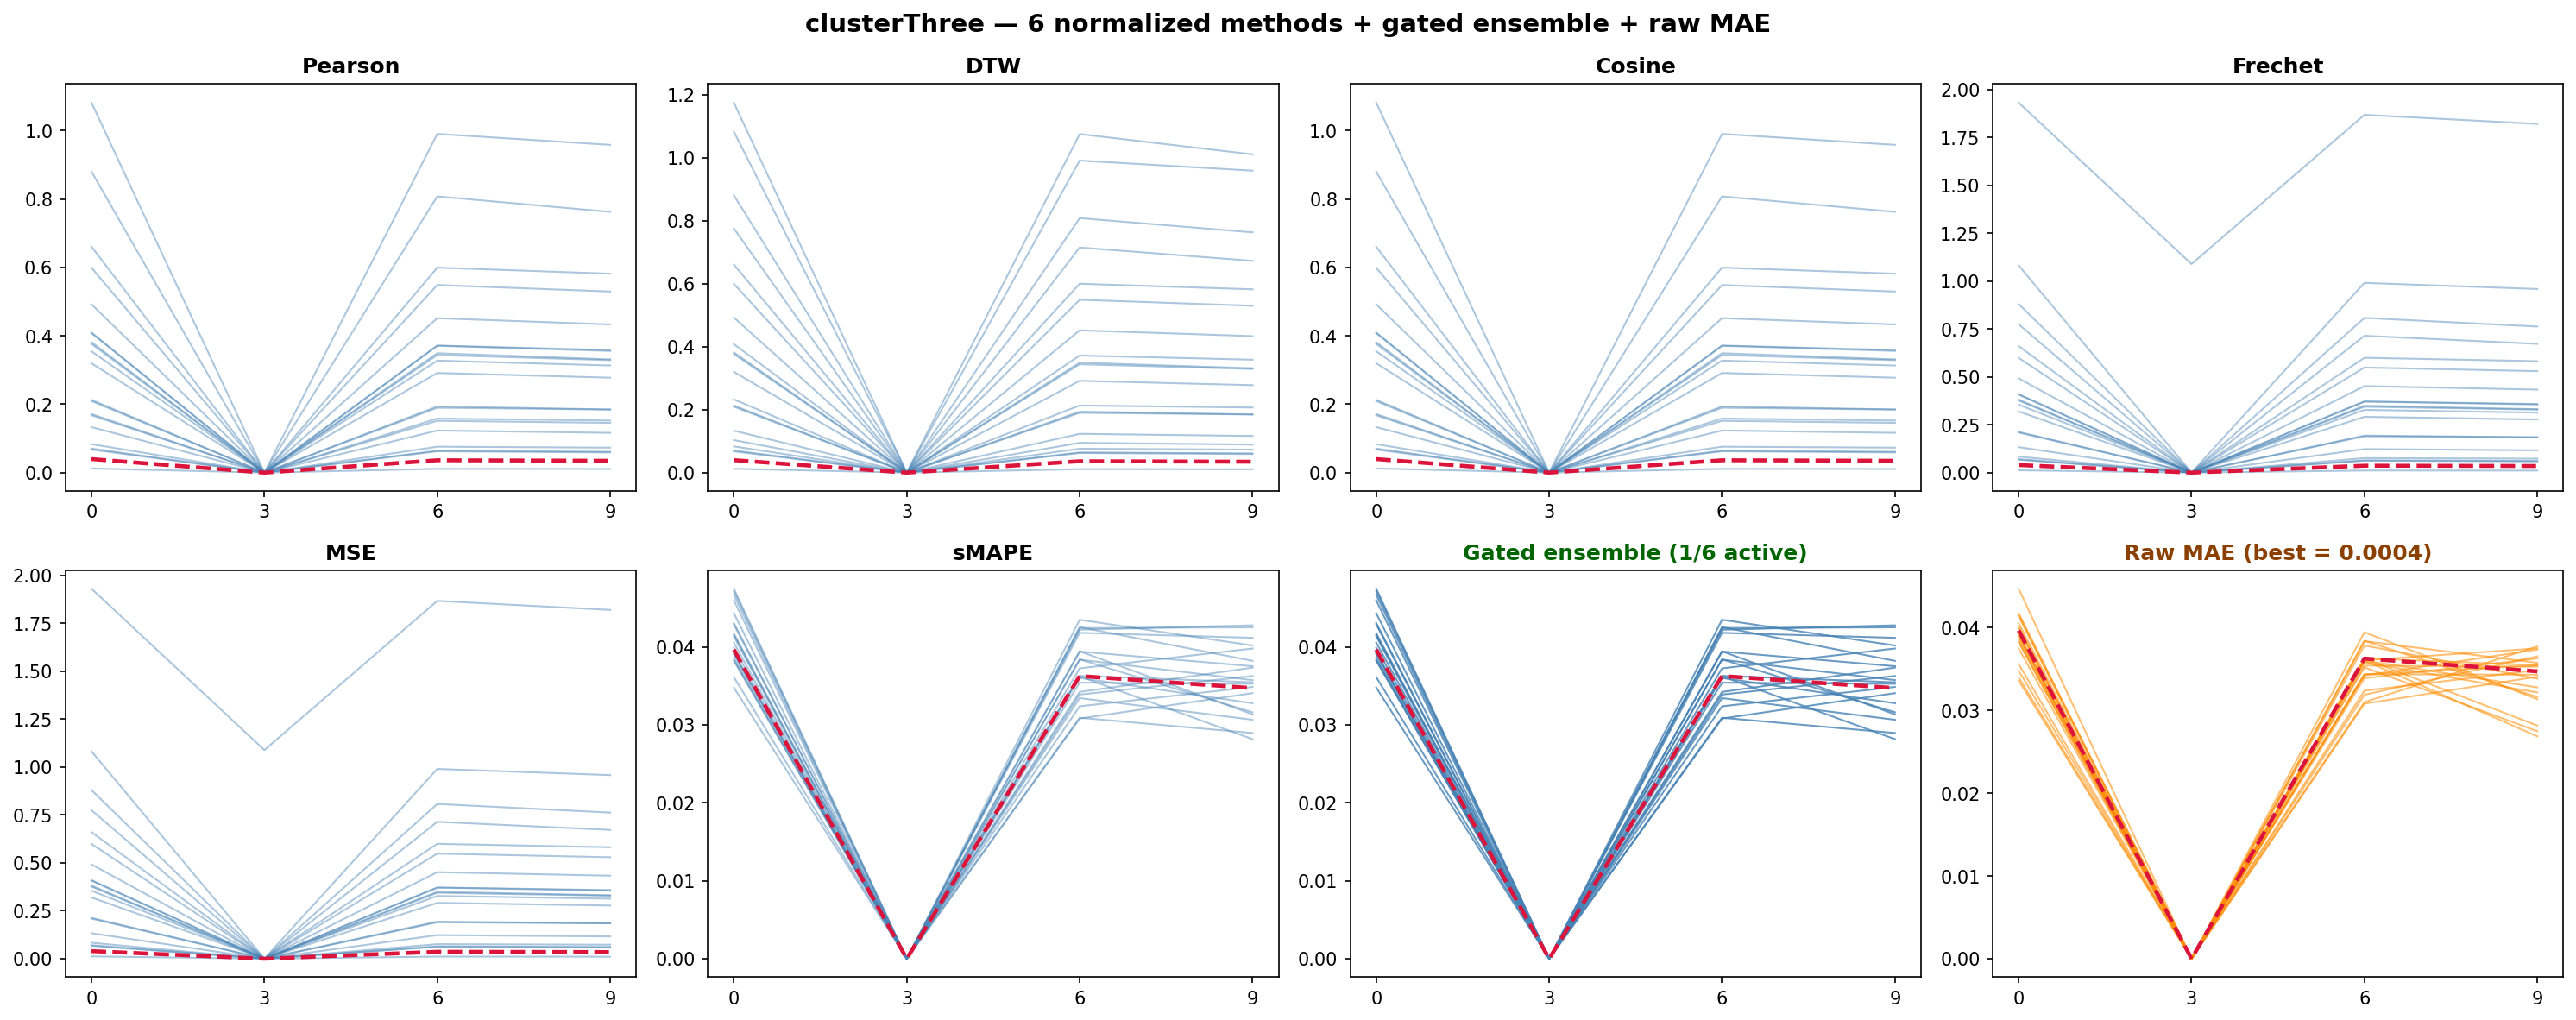
\includegraphics[width=\textwidth,height=0.78\textheight,keepaspectratio]{plots/eightways_clusterThree.png}
\end{center}
\end{frame}

% ------------------------------------------------------------------
\begin{frame}{clusterFour --- Sharp Spike, Large Magnitude}
\footnotesize
7.4\% of genes share \texttt{(+,-,+)}. 5 of 6 normalized methods pick \textit{flat} genes --- normalization erased the spike entirely. Gated ensemble: 6/6 still active --- \textit{the gate didn't catch this failure}. Raw MAE captures the spike-shaped genes for the first time. \textbf{\textcolor{binggreen}{Magnitude uniquely captures the spike at $t=3$.}}
\normalsize
\begin{center}
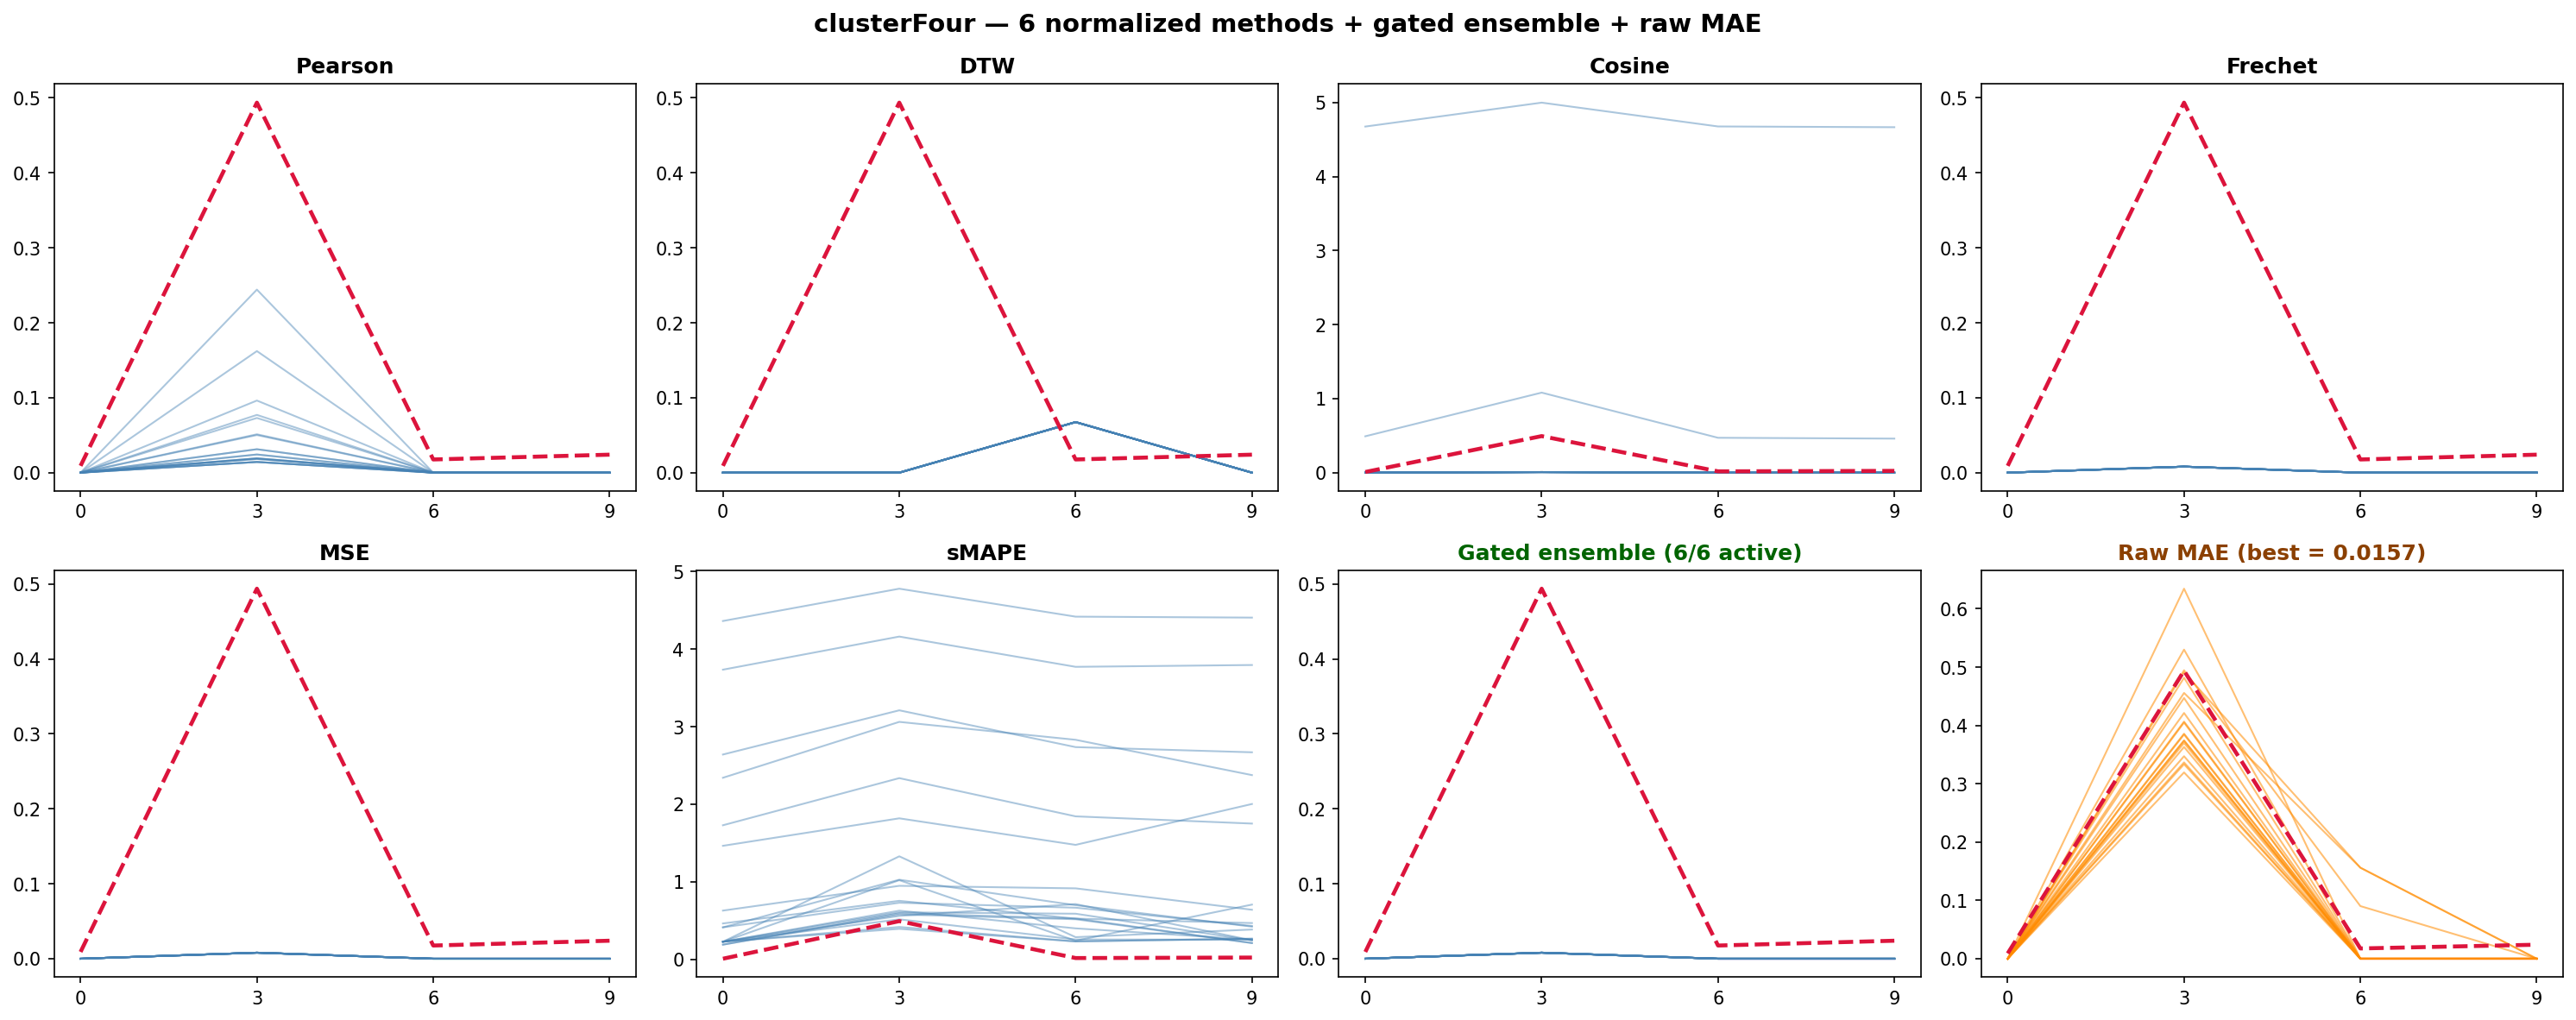
\includegraphics[width=\textwidth,height=0.78\textheight,keepaspectratio]{plots/eightways_clusterFour.png}
\end{center}
\end{frame}

% ------------------------------------------------------------------
\begin{frame}{Question for the Group}
\vfill
\begin{center}
\Large
What does ``similar gene'' mean biologically\\
for these TCR constraint patterns?\\[2em]
\normalsize
Direction of change, or absolute expression level?
\end{center}
\vfill
\end{frame}

% ==================================================================
% Appendix
% ==================================================================
\appendix

\begin{frame}{Appendix --- clusterOne (raw space)}
\begin{center}
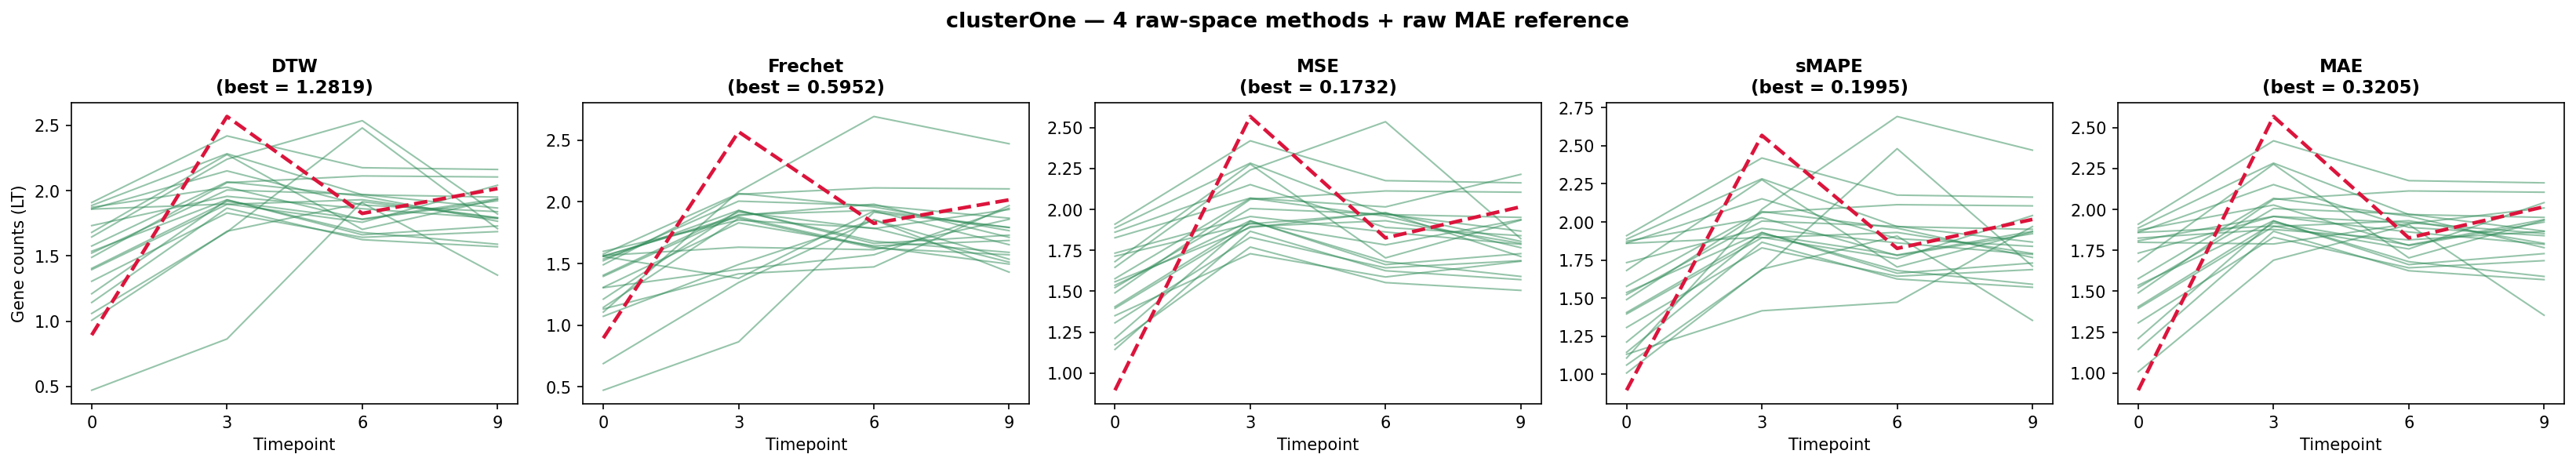
\includegraphics[width=\textwidth,height=0.85\textheight,keepaspectratio]{plots/raw_composite_clusterOne.png}
\end{center}
\end{frame}

\begin{frame}{Appendix --- clusterTwo (raw space)}
\begin{center}
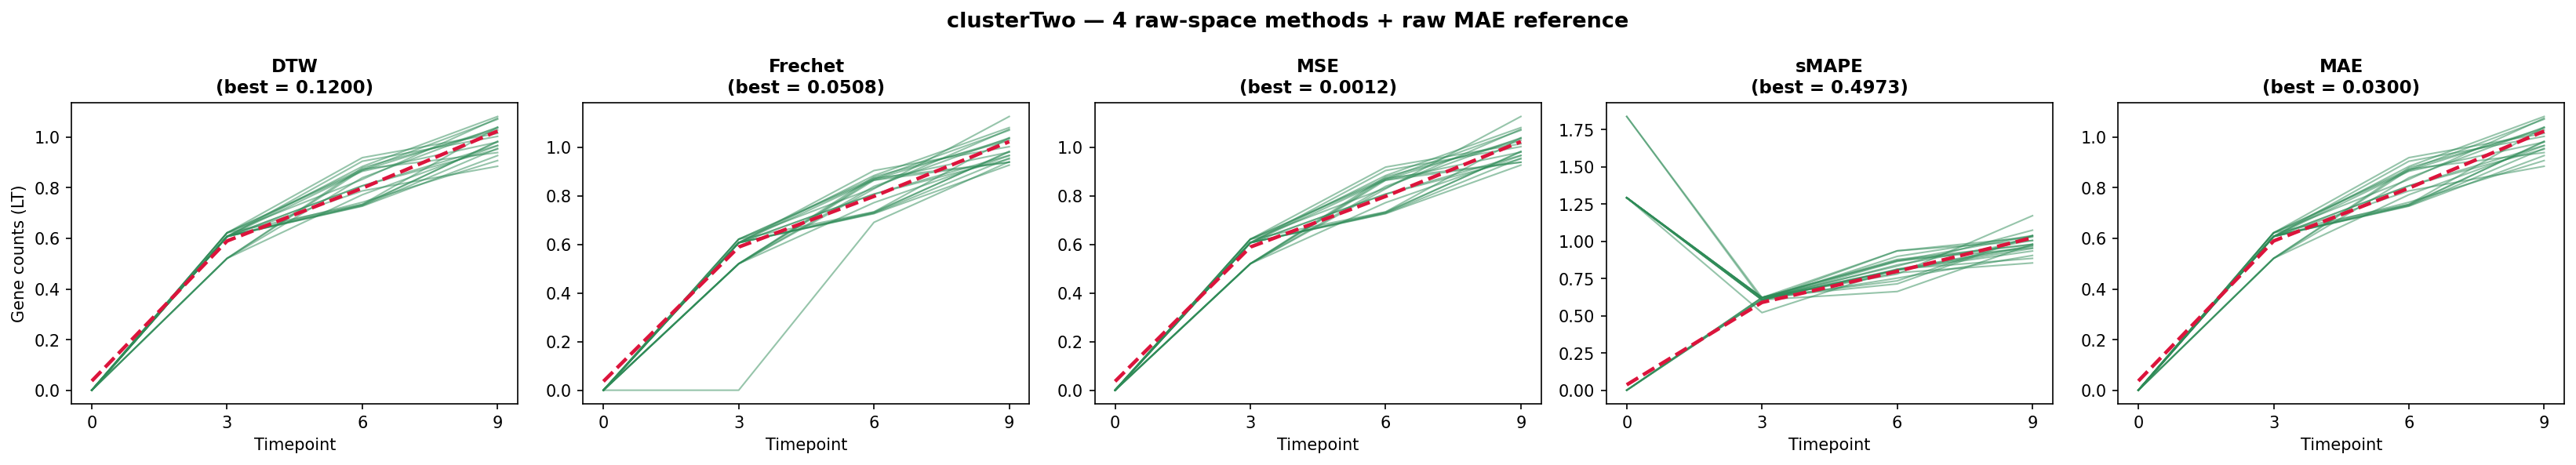
\includegraphics[width=\textwidth,height=0.85\textheight,keepaspectratio]{plots/raw_composite_clusterTwo.png}
\end{center}
\end{frame}

\begin{frame}{Appendix --- clusterThree (raw space)}
\begin{center}
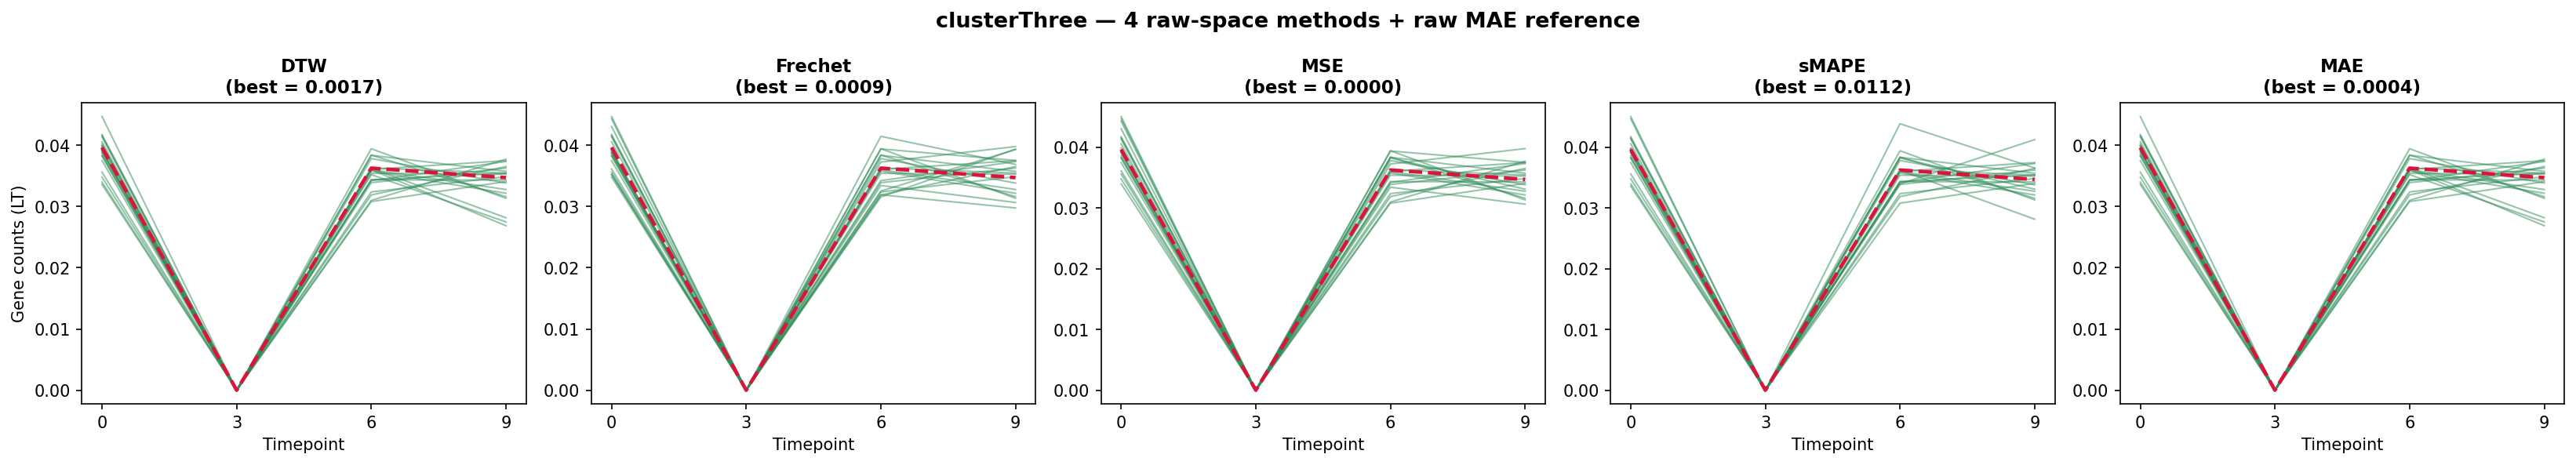
\includegraphics[width=\textwidth,height=0.85\textheight,keepaspectratio]{plots/raw_composite_clusterThree.png}
\end{center}
\end{frame}

\begin{frame}{Appendix --- clusterFour (raw space)}
\begin{center}
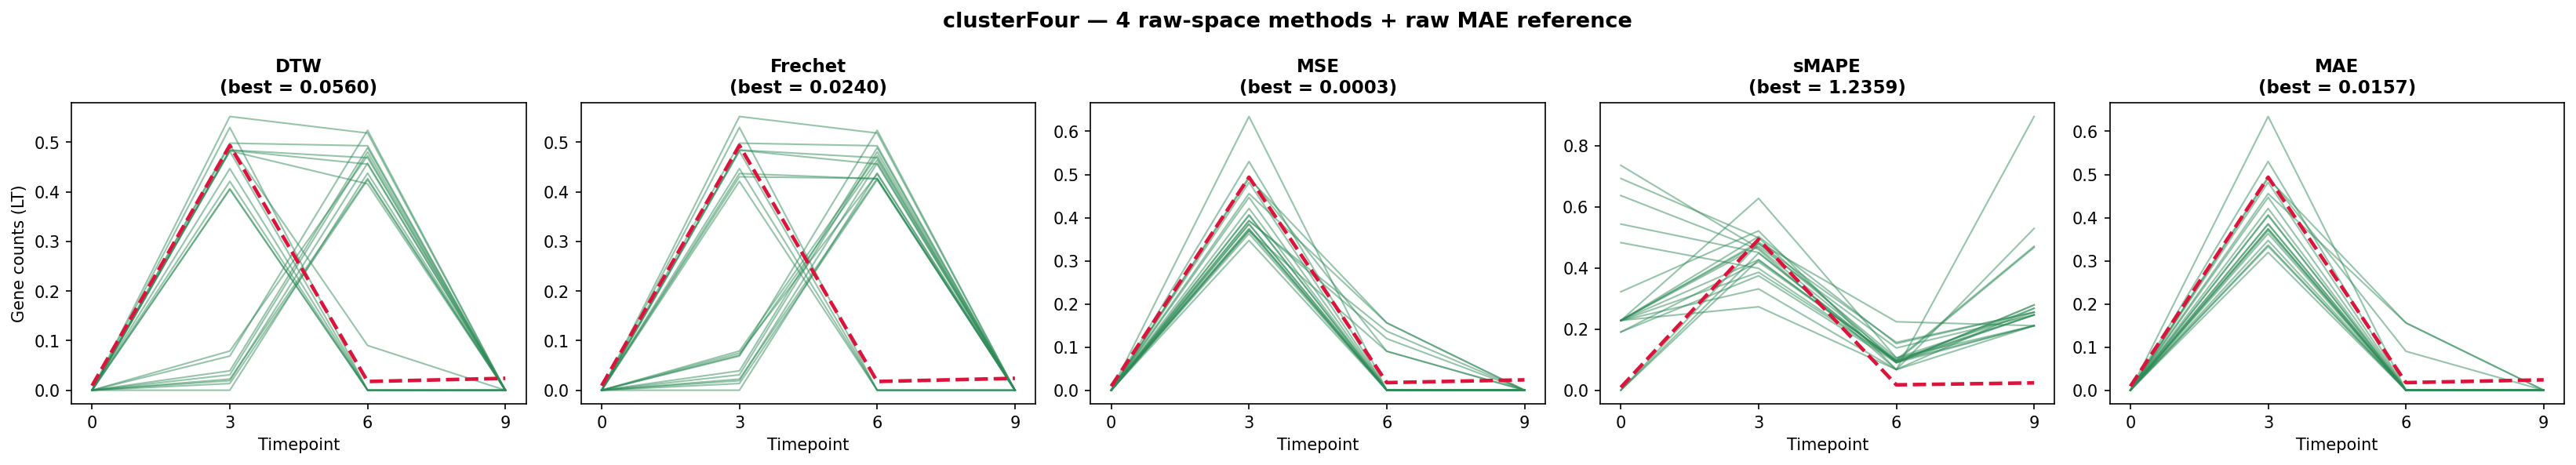
\includegraphics[width=\textwidth,height=0.85\textheight,keepaspectratio]{plots/raw_composite_clusterFour.png}
\end{center}
\end{frame}

\end{document}
